\documentclass{standalone}
\usepackage{graphicx}	
\usepackage{amssymb, amsmath}
\usepackage{color}

\usepackage{tikz}
\usetikzlibrary{intersections, backgrounds}

\definecolor{light}{RGB}{220, 188, 188}
\definecolor{mid}{RGB}{185, 124, 124}
\definecolor{dark}{RGB}{143, 39, 39}
\definecolor{highlight}{RGB}{180, 31, 180}
\definecolor{gray10}{gray}{0.1}
\definecolor{gray20}{gray}{0.2}
\definecolor{gray30}{gray}{0.3}
\definecolor{gray40}{gray}{0.4}
\definecolor{gray60}{gray}{0.6}
\definecolor{gray70}{gray}{0.7}
\definecolor{gray80}{gray}{0.8}
\definecolor{gray90}{gray}{0.9}
\definecolor{gray95}{gray}{0.95}

\begin{document}

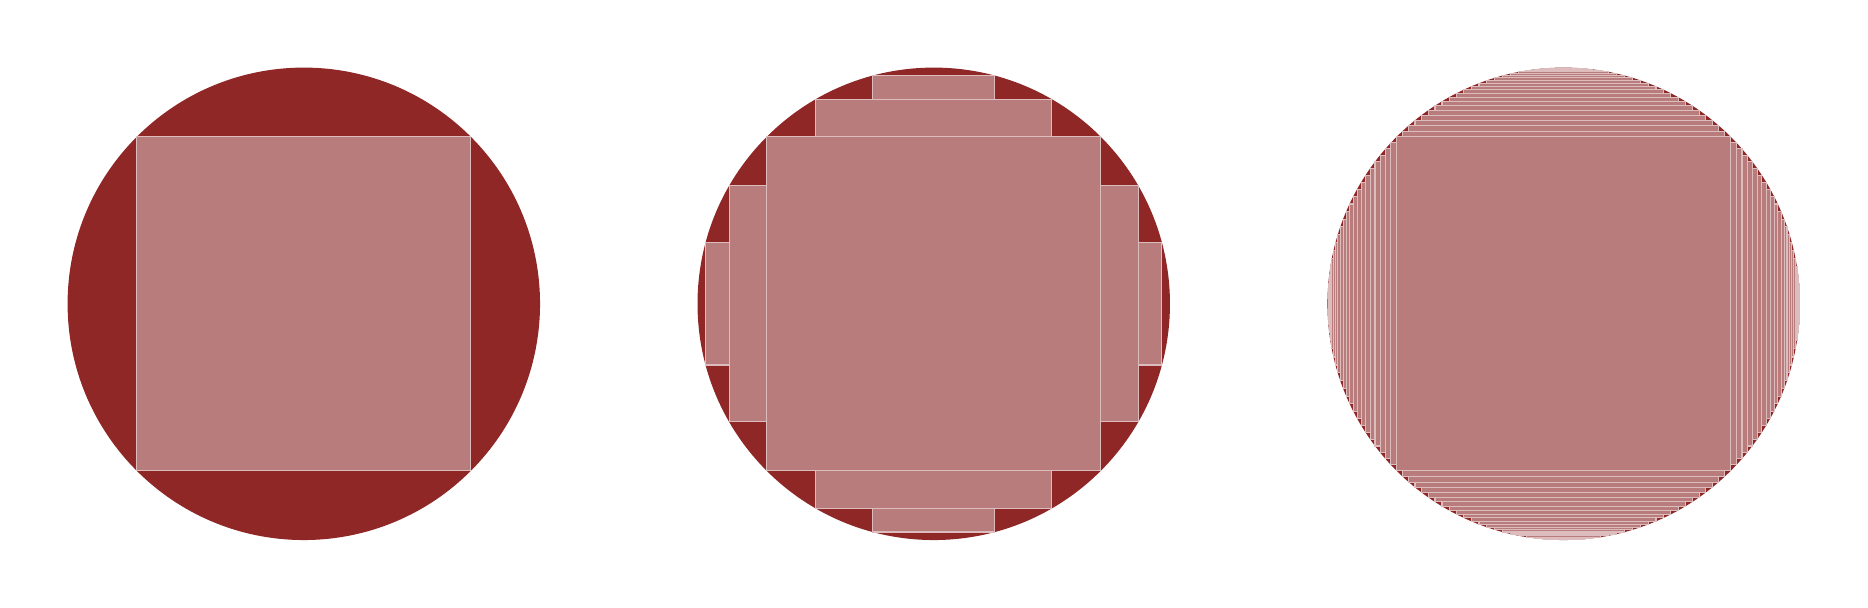
\begin{tikzpicture}[scale=1]
  \pgfmathsetmacro{\r}{3}

  \begin{scope}[shift={(0, 0)}]
    \draw[white] (-3.5, -3.5) rectangle (3.5, 3.5);
    \fill[dark] (0, 0) circle (\r);
    
    \filldraw[fill=mid, draw=light] ({-\r * cos(45)}, {-\r * cos(45)}) 
                         rectangle ({\r * cos(45)}, {\r * cos(45)});
  \end{scope}

  \begin{scope}[shift={(8, 0)}]
    \draw[white] (-3.5, -3.5) rectangle (3.5, 3.5);
    \fill[dark] (0, 0) circle (\r);
               
    \foreach \delta in {30, 15} {
      \filldraw[fill=mid, draw=light] ({-\r * cos(45 + \delta)}, 0) 
                            rectangle ({\r * cos(45 + \delta)}, {\r * sin(45 + \delta)});
      \filldraw[fill=mid, draw=light] (0, {-\r * cos(45 + \delta)}) 
                            rectangle ({\r * sin(45 + \delta)}, {\r * cos(45 + \delta)});
      \filldraw[fill=mid, draw=light] ({-\r * cos(45 + \delta)}, 0) 
                            rectangle ({\r * cos(45 + \delta)}, {-\r * sin(45 + \delta)});
      \filldraw[fill=mid, draw=light] (0, {-\r * cos(45 + \delta)}) 
                            rectangle ({-\r * sin(45 + \delta)}, {\r * cos(45 + \delta)});
    } 
    
    \filldraw[fill=mid, draw=light] ({-\r * cos(45)}, {-\r * cos(45)}) 
                          rectangle ({\r * cos(45)}, {\r * cos(45)});
  \end{scope}

  \begin{scope}[shift={(16, 0)}]
    \draw[white] (-3.5, -3.5) rectangle (3.5, 3.5);
    \fill[dark] (0, 0) circle (\r);
               
    \foreach \delta in {40, 38, ..., 2} {
      \filldraw[fill=mid, draw=light] ({-\r * cos(45 + \delta)}, 0) 
                            rectangle ({\r * cos(45 + \delta)}, {\r * sin(45 + \delta)});
      \filldraw[fill=mid, draw=light] (0, {-\r * cos(45 + \delta)}) 
                            rectangle ({\r * sin(45 + \delta)}, {\r * cos(45 + \delta)});
      \filldraw[fill=mid, draw=light] ({-\r * cos(45 + \delta)}, 0) 
                            rectangle ({\r * cos(45 + \delta)}, {-\r * sin(45 + \delta)});
      \filldraw[fill=mid, draw=light] (0, {-\r * cos(45 + \delta)}) 
                            rectangle ({-\r * sin(45 + \delta)}, {\r * cos(45 + \delta)});
    } 
    
    \filldraw[fill=mid, draw=light] ({-\r * cos(45)}, {-\r * cos(45)}) 
                          rectangle ({\r * cos(45)}, {\r * cos(45)});
  \end{scope}
   
\end{tikzpicture}

\end{document}  